For this case, the numerical simulation is performed for a real 
coronary artery with atherosclerosis whose geometry was obtained 
through an image processing as suggested by Wang et al. (2017) 
\cite{wang2017}. This geometry is particular to each patient 
due to the patient health conditions. As in the previous cases, 
an channel obstruction of 40\% was considered due to atherosclerosis 
and the domain was discretized using 7632 nodes and 14665 linear 
triangular elements. 

\par 
The \ref{velocity evolution real} shows the velocity profile 
in the middle of the channel ($x=5R$). The maximum non-dimensional
 value of the velocity field reaches $u=2.25$. Thus, the 
curved geometry represents a good approximation as seen in 
\ref{velocity evolution curved}, 
such that the difference of maximum non-dimensional velocity value 
is about 2\%.
.

\begin{figure}[H]
     \centering
     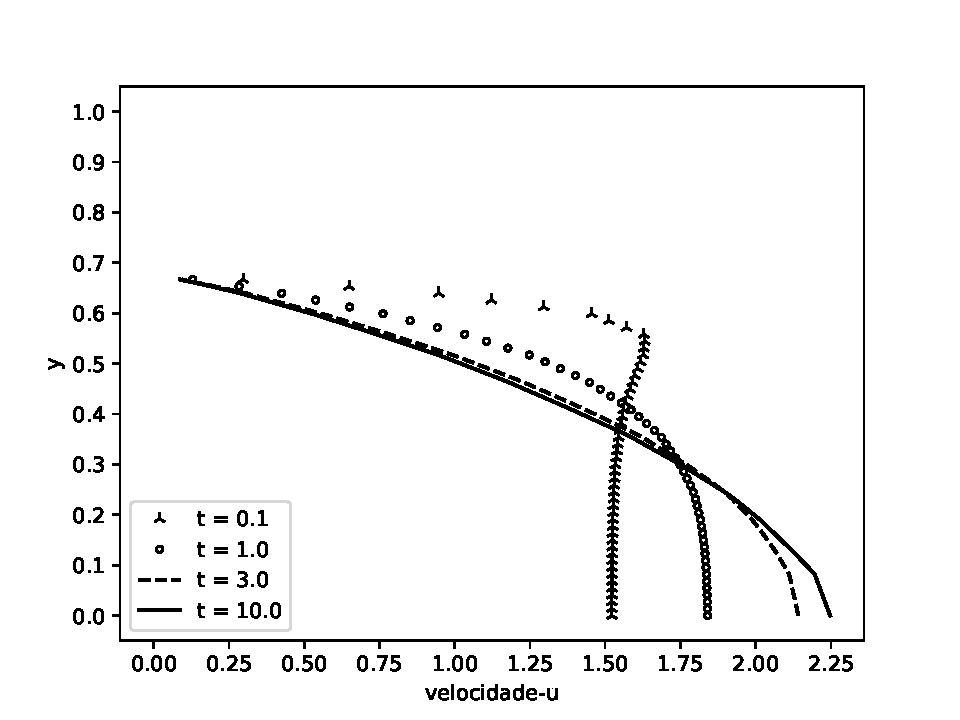
\includegraphics[scale=1]{./02_chaps/cap_solution/figure/vel_Real_evol.pdf}\\
     \caption{The unsteady velocity profile for the real channel.}
     \label{velocity evolution real}
\end{figure}

\newpage
The 
\ref{velocity field real} 
shows the evolution in time and space of the velocity field for half of the
domain The velocity field is represented with non-dimensional values where the red color
refers to the value 
$u=2.25$
and the blue color 
$u=0$
approximately. 
Converting to dimensional
values we have 
$u = 27.0cm/s$
 and 
$u = 0cm/s$ 
respectively.

\vspace{2cm} 
\begin{figure}[H]
     \begin{minipage}{.50\linewidth}
      \centering
      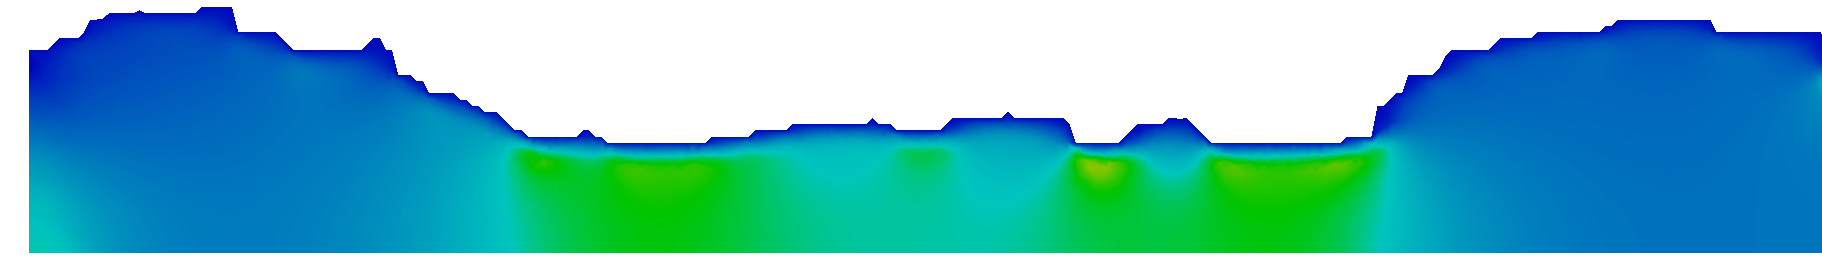
\includegraphics[scale=0.12]{./02_chaps/cap_solution/figure/vel_Real200.png}\\
      t = 0.1
     \end{minipage}%
     \begin{minipage}{.50\linewidth}
      \centering
      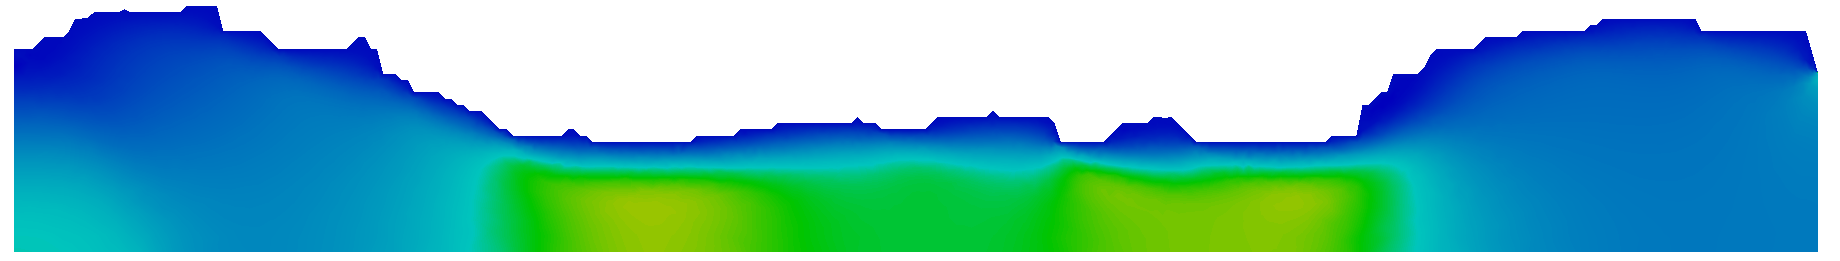
\includegraphics[scale=0.12]{./02_chaps/cap_solution/figure/vel_Real1000.png}\\
      t = 0.5
     \end{minipage}
     \begin{minipage}{.50\linewidth}
     \medskip
      \centering
      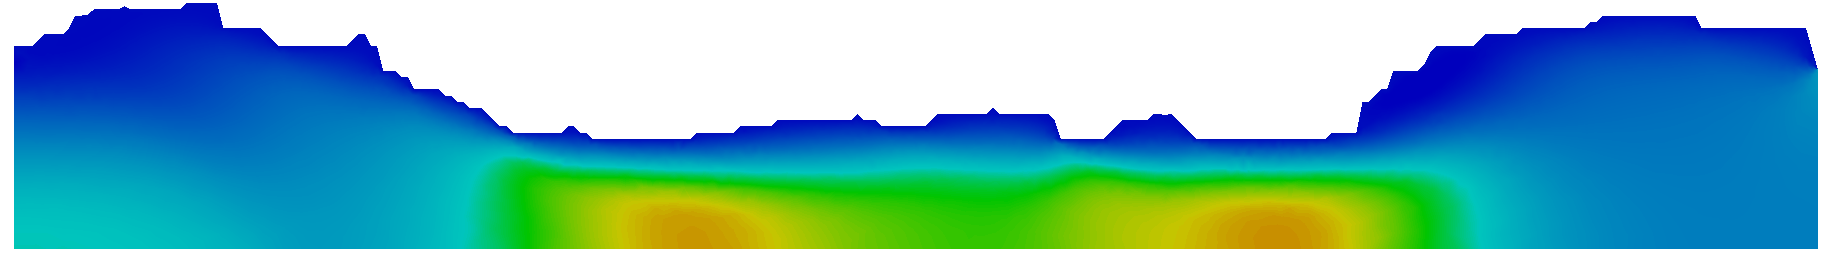
\includegraphics[scale=0.12]{./02_chaps/cap_solution/figure/vel_Real2000.png}\\
      t = 1.0
     \end{minipage}%
     \begin{minipage}{.50\linewidth}
     \medskip
      \centering
      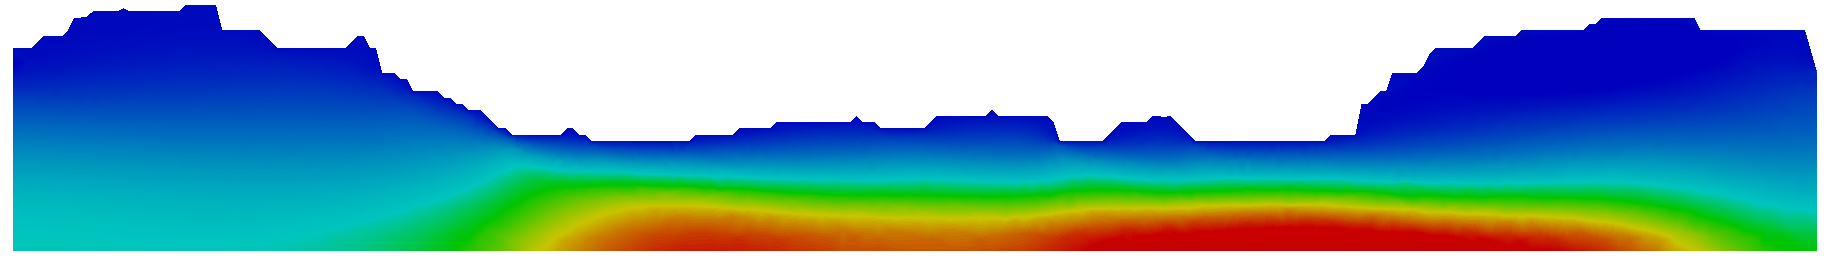
\includegraphics[scale=0.12]{./02_chaps/cap_solution/figure/vel_Real6000.png}\\
      t = 3.0
     \end{minipage}
     \begin{minipage}{.50\linewidth}
      \centering
      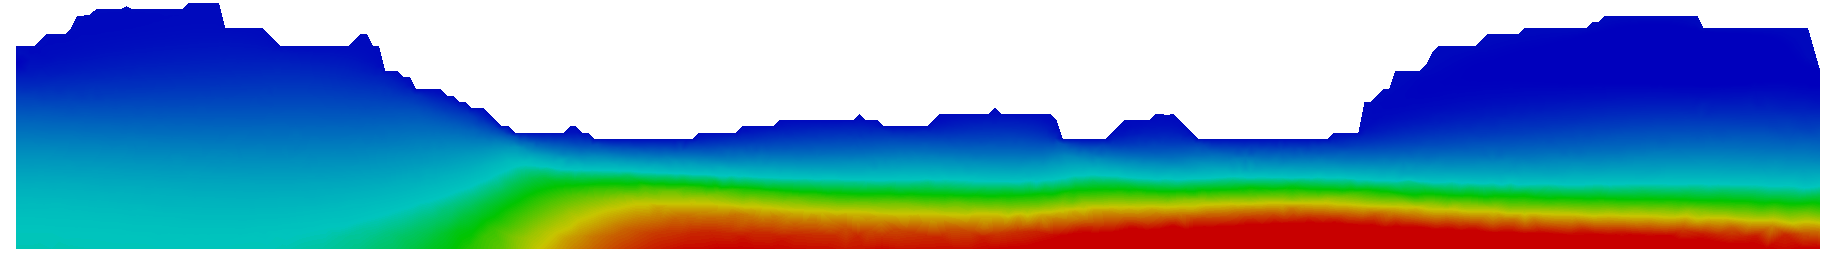
\includegraphics[scale=0.12]{./02_chaps/cap_solution/figure/vel_Real8000.png}\\
      t = 4.0
     \end{minipage}%
     \begin{minipage}{.50\linewidth}
      \centering
      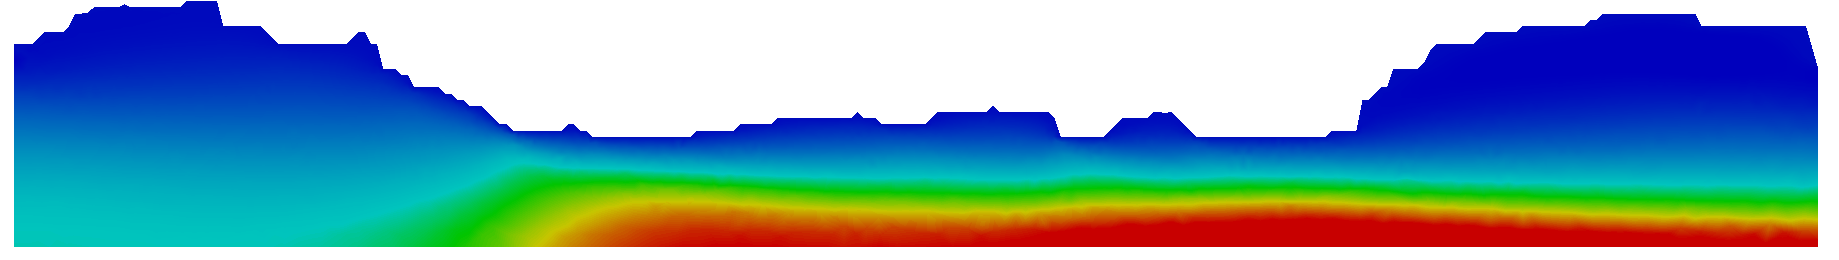
\includegraphics[scale=0.12]{./02_chaps/cap_solution/figure/vel_Real10000.png}\\
      t = 5.0
     \end{minipage}
     \begin{minipage}{.50\linewidth}
     \medskip
      \centering
      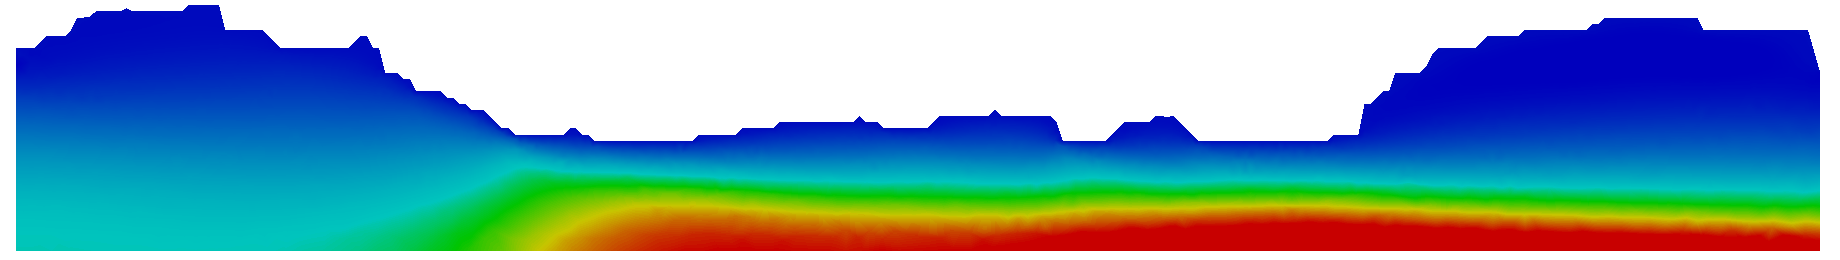
\includegraphics[scale=0.12]{./02_chaps/cap_solution/figure/vel_Real14000.png}\\
      t = 7.0
     \end{minipage}%
     \begin{minipage}{.50\linewidth}
     \medskip
      \centering
      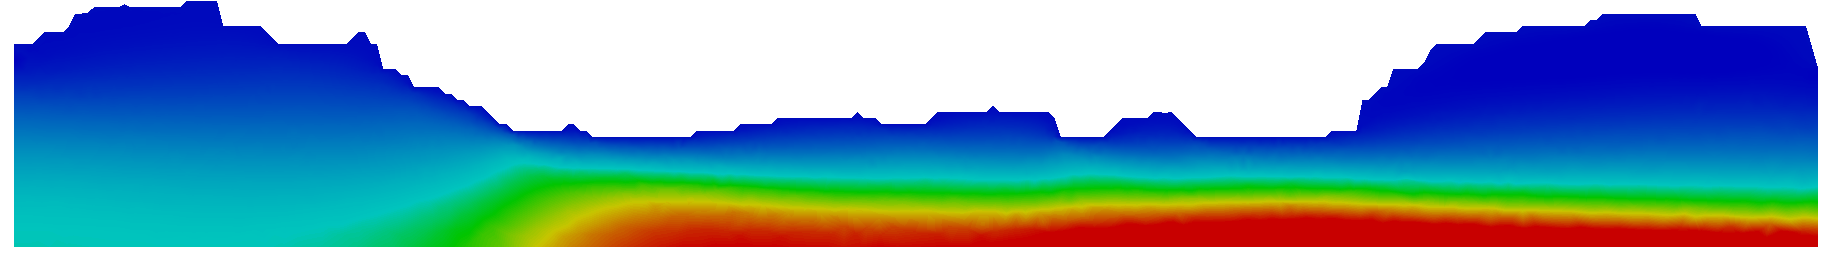
\includegraphics[scale=0.12]{./02_chaps/cap_solution/figure/vel_Real20000.png}\\
      t = 10.0
     \end{minipage}
     \medskip
     \caption{Time and space evolution of the velocity field for real channel.} 
     \label{velocity field real}
\end{figure}

\newpage
